
\chapter{根因分析} % Introduction chapter suppressed from the table of contents

\hypertarget{ux5206ux6790ux4e8bux6545ux6839ux56e0ux4e0aux96c6}{%
\subsection{分析事故根因:上集}\label{ux5206ux6790ux4e8bux6545ux6839ux56e0ux4e0aux96c6}}

北京的某软件开发公司,专门为电信供应商做定制软件开发与运营,比如用短信做些推广活动等。公司希望做过程改进。\\
我:
过程改进的主要目的是帮助企业更好地达成业务目标。你们应该是最清楚自己有哪些不足的,请问你觉得哪些方面有改进空间?\\
总经理:
我不太熟悉技术细节,只能从客户视角来看。例如,去年因为软件的一个错误导致客户损失了几十万元,我立即在公司内部开会,希望找出根因,最后发现是因为某个开发人员粗心大意,在编码时把两行数字搞错了,在测试人员针对这项功能进行测试时,虽然收到短信了,但并没有仔细看短信的内容,也就没有发现这个缺陷,测试通过了。这起事故不仅招致了公司的经济损失,更影响了客户对我司的信任度,也影响公司在行业内的口碑。\\
我: 公司采取了哪些纠正措施?\\
总经理:
之后我们加强了对代码的评审工作,要求这类代码都需要经过主管审查,还增加了相应的惩罚措施,
如果再次发生同类事件,项目经理和部门负责人都要承担连带责任。\\
我:采取这个措施之后,效果如何?\\
总经理:很好,大家都注意了,到现在都还没有再发生同类的问题。

\begin{description}
\item[]
\begin{description}
\tightlist
\item[]
= = =
\end{description}
\end{description}

你认为以上的纠正措施能避免同类问题的再次发生吗?\\
你可能赞同以上事故的主因是人员疏忽,但很多事故的主因其实不仅仅是人员疏忽。

\hypertarget{ux9999ux6e2fux5357ux4e2bux6d77ux96be}{%
\subsection{香港南丫海难}\label{ux9999ux6e2fux5357ux4e2bux6d77ux96be}}

\framebox{%
\begin{minipage}[t]{0.97\columnwidth}\raggedright
2012年10月1日晚上8时,任职港九小轮的黎细明驾驶海泰号(注)由中环出发前往南丫岛榕树湾。15分钟后,任职港灯的周志伟驾驶南丫四号从榕树湾出发,接载港灯员工及亲友到维港观赏国庆烟花。两船于8时20分相撞,南丫四号船尾迅速沉没,造成39人遇难。

(注:海泰号是大型喷射双体船,速度与载客量都远比南丫四号高。)

\strut
\end{minipage}}

南丫四号船尾沉没,消防处安排潜水员紧急救援:\\
%\href{文件:LammaAccidentScreenshot_2023-06-01_194248.jpg}{550px}

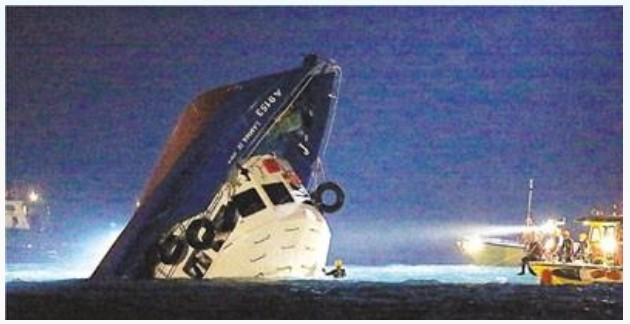
\includegraphics[width=6cm]{LammaAccidentScreenshot_2023-06-01_194248.jpg}

黎细明(左,56岁),小二文化程度,1982年任职小轮公司,2008年成为船长。\\
%\href{文件:CaptainScreenshot_2023-06-01_195518.jpg}{200px}

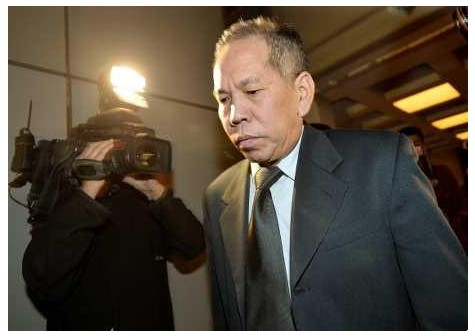
\includegraphics[width=6cm]{CaptainScreenshot_2023-06-01_195518.jpg}

%\href{文件:Captain2Screenshot_2023-06-01_195805.jpg}{150px}\\

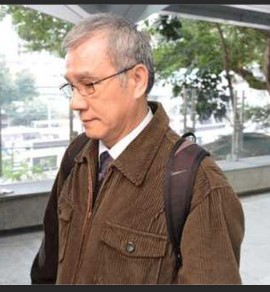
\includegraphics[width=6cm]{Captain2Screenshot_2023-06-01_195805.jpg}

周志伟(58岁),小六文化程度,已婚,育有两女,1974成为海员,1993年开始担任船长。

\framebox{%
\begin{minipage}[t]{0.97\columnwidth}\raggedright
2015年,开庭审判两船长:\\
周:碰撞发生前,南丫四号曾右3转度避撞,但海泰号违规左转3度,且海泰号船速较快及操控性较高,故南丫四号的避撞措施均被海泰号的相反举动抵消。

黎:造成大量乘客死亡的原因是南丫四号船身有问题,包括部分船舱并非水密舱等,而且海上的雾灯及其他背景灯光也影响了我的视线,难以观察到南丫四号。

专家:海泰号没有根据"国际海上避碰规则"右转,反而左转3度,属"极度危险",南丫四号虽曾按规则向右转,但"幅度太小、转得太迟"。

\begin{itemize}
\tightlist
\item
  陪审团以7比2 裁定黎细明误杀罪成立,法官判入狱8年
\item
  陪审团以8比1 裁定周志伟误杀罪不成立,但危害他人在海上安全罪以7比2
  裁定罪成,法官判入狱6个月
\end{itemize}
\strut
\end{minipage}}


你赞同两位船长的失职是本次海难的根因吗?

政府经过3年多的事件调查,最终做出调查报告。报告显示,在海难中沉没的南丫四号,从设计到验收,每个环节都存在纰漏,每个环节都有出错,例如包括:

\begin{itemize}
\tightlist
\item
  没有安装水密门 (导致南丫四号在碰撞另一艘船之后,迅速沉没)
\item
  座位的螺丝松动
  (导致撞船后,因船尾沉没水中,所有座位都松脱,跌到船尾,影响乘客逃生)
\item
  没有儿童救生衣等
\end{itemize}

因此导致南丫四号在碰撞海泰号之后,迅速沉没,并且导致罹难人数众多,政府展开内部调查,怀疑海事处有十七名职员应负责任。

除了南丫四号的问题,你是否觉得小轮公司也应负责任,例如:

\begin{itemize}
\tightlist
\item
  对船长的培训/监督是否足够
\item
  是否有定期检查船上救生设备
\end{itemize}

你可能要反驳,像``南丫四号''这类小型船,预算少,所以关注度、监控度都低,如果是大型项目应该不会出现这类纰漏事故,请看看美国NASA的太空穿梭机(Space
Shuttle)计划因发生了两次致命的事故,最终被叫停的案例。

\framebox{%
\begin{minipage}[t]{0.97\columnwidth}\raggedright
太空穿梭机灾难 (Space Shuttle disasters) \\
1986:挑战者号(Challenger),挑战者号航天飞机升空后,于发射后的第73秒爆炸,机上7名宇航员全部罹难。(
相关视频可以在网上搜到)\\
2003: 哥伦比亚号
(Columbia)航天飞机在返回地球时,因为左翼的隔热保护胶在十六天前升空时被固体火箭助推器外层脱落的乳胶击破损坏,导致航天飞机返航时进入大气层的第1000秒钟,在35,000米高空因过热解体,7名宇航员全部罹难。\\
Sally RIDE 在2003哥伦比亚号灾难事故调查回顾说
:我很诧异这两次事故的原因非常相似 (她也是挑战者号事故调查组员),86
年引起挑战者灾难的陋习又再出现 :
为了赶上计划升空日期,而忽略了之前性能报告的发现,没有注意前线技术工程人员提出的安全隐患,也缺乏安全保障措施。其实从哥伦比亚号在1981年首次升空开始,每次都有出现升空时燃料缸外的保护乳胶掉落的事故,但管理层一直都没有关注,工程师因为赶进度,每次升空前,都没有时间预先处理好。

%\href{文件:2_Space-Shuttle-Columbia-team.jpg}{250px\textbar{}有框\textbar{}左\textbar{}图3:
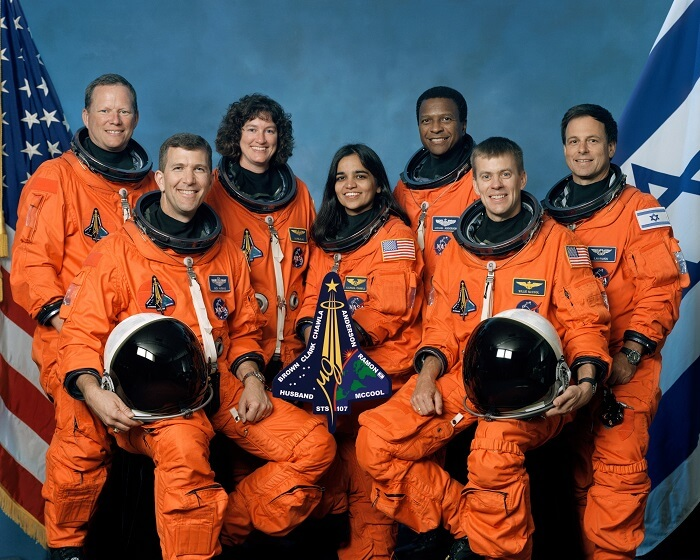
\includegraphics[width=6cm]{2_Space-Shuttle-Columbia-team.jpg}
%7名哥伦比亚号宇航员}\\
\strut
\end{minipage}}

如果管理层、工程师只关注项目的成本与进度,忽略了质量与安全,便会导致灾难。

其它很多相似的航空或海上灾难,虽然当事人(如船长)的失误引发了事故,但这并非根因,背后系统的不足才是主因。

上面总经理的纠正措施能避免同类问题再次出现吗?\\
不一定。因为已经导致公司极大的损失,而且引发了高管的关注,开始的时候大家会注意,但并不能长久,因为这仅仅依赖于个人的习惯,很可能在几个月后还会再次发生。

\hypertarget{ux6839ux56e0ux5206ux6790ux7684ux4e3bux8981ux5143ux7d20}{%
\subsection{根因分析的主要元素}\label{ux6839ux56e0ux5206ux6790ux7684ux4e3bux8981ux5143ux7d20}}

如果想挖掘系统的不足,便必须找出根因,根因分析主要包含那些元素?可参考CMMI模型的根因分析(Causal
Analysis \& Resolution CAR):

%\href{文件:CMMIHM_02.png}{文件:CMMIHM 02.png}

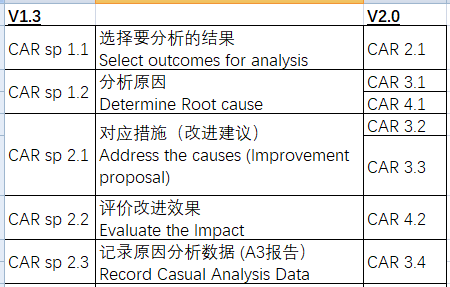
\includegraphics[width=6cm]{CMMIHM_02.png}

\begin{enumerate}
\tightlist
\item
  利用二八原则识别引起大部分问题的最主要因素
\item
  分析背后的主要原因
\item
  对应改进措施
\item
  判断改进效果
\item
  总结成根因分析报告
\end{enumerate}

可参考附录A:
"绅士俱乐部过程改进"了解QC圈如何按意识根因分析元素完成为期七个月的过程改进。本章附件也有二八原则与帕累托图的介绍。但不要误以为只要使用各种根因分析方法,如帕累托图、鱼骨图等,就能做好根因分析.

\hypertarget{ux6839ux56e0ux5206ux6790ux8befux89e3ux6848ux4f8b}{%
\subsubsection{根因分析误解案例}\label{ux6839ux56e0ux5206ux6790ux8befux89e3ux6848ux4f8b}}

\framebox{%
\begin{minipage}[t]{0.97\columnwidth}\raggedright
某公司过程改进组(共4人)分析以往一年项目,做根因分析,希望改进交付的质量,减少交付验收时的缺陷数。

%\href{文件:Epg-car3.1-1.png}{400px}\\
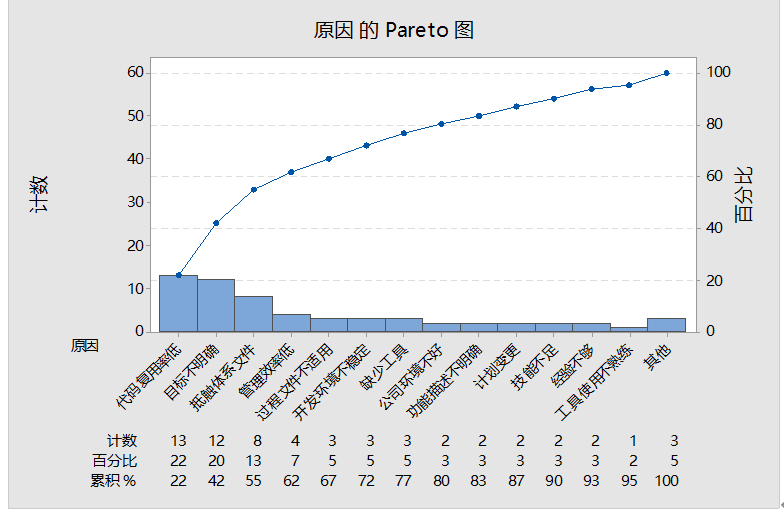
\includegraphics[width=6cm]{Epg-car31-1.png}

\strut
\end{minipage}}

我:请问这帕累托图的依据?\\
组长:针对客户缺陷密度较高的现状,我们做了敏感度分析。发现需求引入的缺陷数跟它相关性最高,我们接下来就用鱼骨图分析,四个人一起头脑风暴,识别出以下十几项主要的原因种类,然后我们就按每人三票,各自单独投票得出这个排序,然后我们就依据二八原则选择了头三项原因是主要的对象,然后我们根据这三项原因发现,这些项目是导致需求缺陷的原因,包括流程图画不好等。

我听完以上根因分析故事,便在投影仪投出以下某机场某年导致航班延误的原因统计表,问项目经理:``假如你是顾问团队,要为机场管理层高层分析导致航班延误的主因并提出改进方案你会怎么利用二八原则画帕里托图?''

\begin{description}
\item[]
\begin{description}
\tightlist
\item[]
香港启德国际机场1996年航班延误统计:
\end{description}
\end{description}

%\href{文件:CRairportDelayScreenshot_2023-06-02_191306.jpg}{600px}
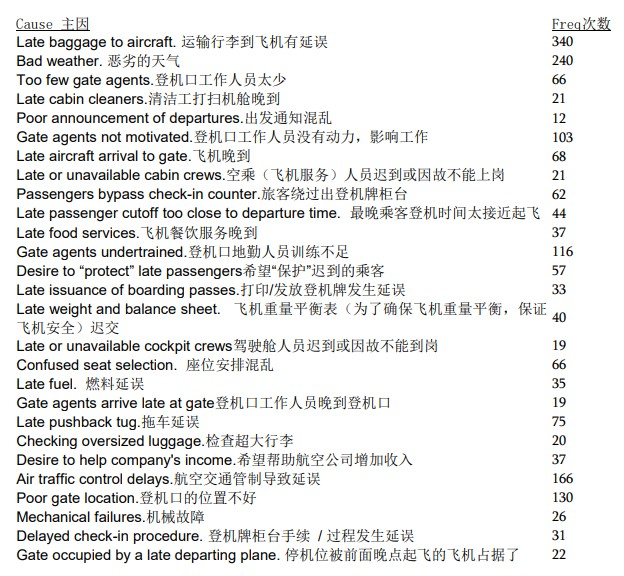
\includegraphics[width=6cm]{CRairportDelayScreenshot_2023-06-02_191306.jpg}


然后我解释:\\
我们不应直接把几十条原因,按每条原因对问题的影响度,从最高排到最低做帕累托图,而应先把原因进行分类。用上面机场延误为例,比如,哪些是不可抗力的天然原因(如天气原因),哪些是跟闸口管理相关的问题,那些是跟机场打印登机牌相关等,例如,如果识别出是跟闸口管理类的问题最多,后面便针对这进一步分析根因。分组才有针对性、有意义。

你们的分类,帕累托图依据的``数据'',都只是用数字形式表达你们头脑风暴的主观判断,
所以你用这种帕累托图其实跟直接用头脑风暴做出做出的结论没什么差异,只是你们用了投票数据使结果看起来``量化''了,其实是没有客观数据支撑。

例如,你们的分类有问题:
例如,只有``功能描述不明确'',难道``非功能需求描述不明确''(如性能、安全性等)就不需要考虑吗?\\
你们现在的分类有不少是重复的,同样一个问题有可能归属于两个、三个分类。

你们度量操作定义有问题,例如,你是如何根据历史项目的数据去判断哪些原因归属于``功能描述不明确''?

如果想做好,应该预先按你们想要解决的问题,识别出相关的度量项,然后针对这些度量项,例如,缺陷,定义如何分类(详见附件``二八原则与数据分类'')并收集数据后,做分析。有了客观的数据分析,才是你们根因分析的第一步。

\begin{description}
\item[]
\begin{description}
\tightlist
\item[]
= = =
\end{description}
\end{description}

我:你们现在的找出的其实并非根因,只是浮在水面上的现象,你们有听过5W吗?\\
组长:有, What When ..\\
我:不,你说的是5W+1H
,5W是五个为什么(why),所以你们应一直追问,才能更好地识别出背后的主因,并针对主因采取纠正措施,才能避免同类问题重复发生。\\
我继续向他们讲述丰田汽车大野耐一先生的5W故事。(详见附件``大野耐一先生5Why例子'')

除了通过问``为什么''之外,模型(例如 CMMI, XP
极限编程等)也可以帮你们更全面地找出根因。
很多原因会导致项目延误。``功能描述不明确''可能只是其中一个原因,例如:

\begin{itemize}
\tightlist
\item
  利用检查单做好需求评审
\item
  与干系人(客户)确认需求
\end{itemize}

如果能做好这些,即可帮助团队确保需求质量,减少项目延误,以上两条都是
CMMI 里的最佳实践,所以模 型可以帮助团队更全面地看问题。

\hypertarget{ux600eux6837ux624dux80fdux505aux597dux6839ux56e0ux5206ux6790}{%
\subsubsection{怎样才能做好根因分析}\label{ux600eux6837ux624dux80fdux505aux597dux6839ux56e0ux5206ux6790}}

从前面各例子看到,有些团队没有根因分析的意识 :
不理解核心思路,只是表面``做''了根因分析的步骤,其实未找到根因。所以,要做好便必须利用培训,提高大家的根因意识。大家从以下日本回国技术总监的故事可以更好理解什么是``根因意识''。

\hypertarget{ux6280ux672fux603bux76d1ux7ecfux9a8cux4e4bux8c08}{%
\subsection{技术总监经验之谈}\label{ux6280ux672fux603bux76d1ux7ecfux9a8cux4e4bux8c08}}

\framebox{%
\begin{minipage}[t]{0.97\columnwidth}\raggedright
总监之前一直在日本带领开发团队,十年前回大陆。最近为他们做过程差距分析,总监开车送我去机场时分享他的日本经历。\tabularnewline
\strut
\end{minipage}}

你说我们团队没有找出真正根因,我非常赞同。日本人在根因分析方面做得特别好。我之前在日本工作,带领小组做开发,当时我们团队共5人,有2位来自大陆,其他是本地人,有一次,因为我们开发计算公积金出错,QA一直追问问题的原因。当时我还没有找出根因的概念,不明白QA的意图,以为只是问责,希望找个人背锅。其实他们确实是希望找出问题的源头,避免同类问题再发生。当时主管追问原因,要求我发问题报告。我的报告只说了一些开发问题,人员经验不足等。主管一直追问为什么。``如果你说培训不足,你有什么相关的培训计划来避免?''我回答不上来。最后发现,原来是日本计算方法和大陆不同,他们不四舍五入,导致我们两位大陆开发人员的计算便和本地的不同。
很多大陆工程师没有根因分析概念,认为质量依靠个人保证,``我负责,有问题我承担''。日本人不是这个思路,他们希望挖掘到问题的根本原因并避免。后面我回国发展,开始时兼职做咨询工作,帮一位老朋友看看某软件开发公司团队的问题,发现很多大陆团队对质量方面的要求远远不如日本,很不习惯。

\framebox{%
\begin{minipage}[t]{0.97\columnwidth}\raggedright
日本产品质量\\
98年,我在香港富士通工作,试图在香港市场推富士通的服务器,富士通服务器跟美国太阳(SUN)匹配(compatible),但价位反比美国太阳服务器高,一直想不出什么原因。后来我去东京出差,发现原来日本公司,例如富士通,对质量特别有要求,产品测试设计等都要通过很多关卡,才可以出厂。有些富士通在澳大利亚的工程师就不明白为什么总公司要求这么苛刻,需要不断测试,觉得浪费资源。他们不清楚原来日本本土客户对质量要求特别高,无论是消费品或电子产品,如果达不到高水平质量要求,基本上卖不出去。富士通公司电子产品以满足本土市场为主,所以必须有很高的质量要求。

客户(甲方)是否对质量有高要求也是促进产品质量的重要因素。\strut
\end{minipage}}

所以如果公司高层没有产品质量的要求,单靠团队学习根因分析技巧不会有改进效果。

\hypertarget{ux7ed3ux675fux8bed}{%
\subsection{结束语}\label{ux7ed3ux675fux8bed}}

根因分析包括下图各主要元素:

%\href{文件:微信截图_20230707090950.png}{600px\textbar{}无}

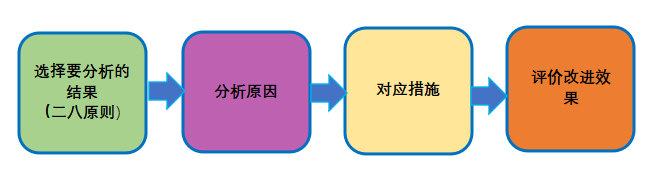
\includegraphics[width=6cm]{微信截图_20230707090950.png}

从上面案例,大家看到如能用好根因分析,应可帮助团队避免同类问题重复发生,帮团队提升。

但要真正做好根因分析不能单靠学理论与方法,必须利用实际数据让团队成员动脑筋和讨论,才能真正用好根因分析,取得效果。

下一章,我们探索针对软件开发如何利用根因分析做好过程改进。

\hypertarget{ux9644ux4ef6}{%
\section{附件}\label{ux9644ux4ef6}}

\hypertarget{ux4e8cux516bux539fux5219ux4e0eux6570ux636eux5206ux7c7b}{%
\subsection{二八原则与数据分类}\label{ux4e8cux516bux539fux5219ux4e0eux6570ux636eux5206ux7c7b}}

帕里托(Pareto)
,16世纪意大利威尼斯人,他发现虽然威尼斯很富有,但财富并非平均分布,80\%财富在20\%手里,他也发现很多其他分布都非平均。

%\href{文件:ToolsParetoScreenshot_2023-06-02_191628.jpg}{400px}

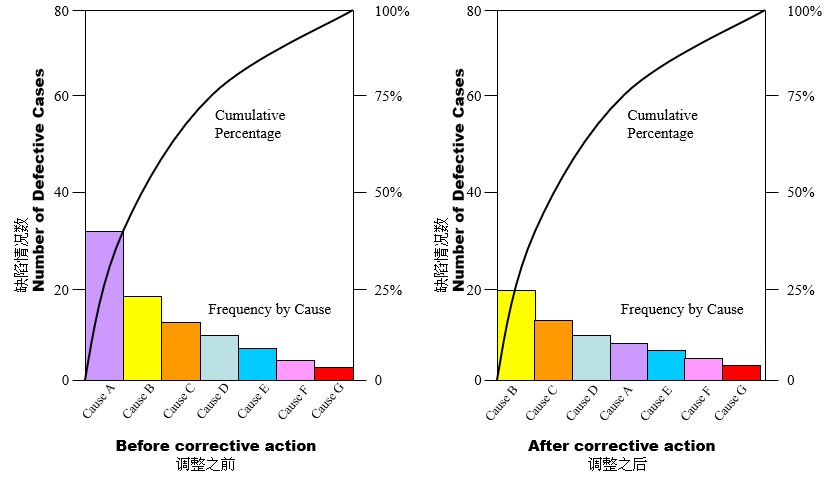
\includegraphics[width=6cm]{ToolsParetoScreenshot_2023-06-02_191628.jpg}

因为过程改进需要公司额外的资源投入,必须有针对性地找出最容易取得改进效果的原因,才可能拥有最大的成功机会。所以,应该利用二八原则去识别影响最大的几个因素.
以上图为例,原本A类问题出现最多,针对这类问题做过程改进之后, A
类问题就少了很多,下一轮便应针对最多的B类问题做改进。

有些人以为,只需要对某个维度做分析即可,并没有从多个维度进行分析

例如,某纸制产品工厂会计数据显示,八成的产品问题相关成本都归属于5类,例如:质量不合格、赔偿、售后现场服务等(共有20类)。
针对5类中最大的一类质量不合格,
发现里面八成的成本都由于六个产品引起(共有50个产品)
针对这六个产品把成本按缺陷种类细分,发现B产品断裂缺陷的成本最高,
我们就应该针对这一问题研究如何改善。

%\href{文件:Ar2_缺陷类型造成的损失.jpg}{文件:Ar2 缺陷类型造成的损失.jpg}

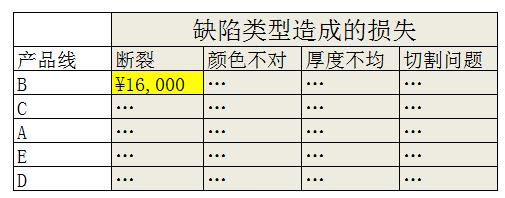
\includegraphics[width=6cm]{Ar2_缺陷类型造成的损失.jpg}

\hypertarget{ux5927ux91ceux8010ux4e00ux5148ux751f-5-why-ux5b9eux4f8b}{%
\subsection{大野耐一先生`` 5 Why
''实例}\label{ux5927ux91ceux8010ux4e00ux5148ux751f-5-why-ux5b9eux4f8b}}

有一次,大野耐一先生见到生产线上的机器总是停转,虽然修过多次但仍不见好转,便上前询问现场的工作人员。\\
(1-Why)问:``为什么机器停了?'' 答:``因为超过了负荷,保险丝就断了。''\\
(2-Why)问:``为什么超负荷呢?'' 答:``因为轴承的润滑不够。''\\
(3-Why)问:``为什么润滑不够?'' 答: ``因为润滑泵吸不上油来。''\\
(4-Why)问:``为什么吸不上油来?''答: ``因为油泵轴磨损、松动了。''\\
(5-Why)问: ``为什么磨损了呢?'' 答:
``因为机器打磨金属零件,空气混进了铁屑等杂质,并掉进机器油缸里。''\\
经过连续五次不停地问``为什么'',找到问题的真正原因(润滑油里面混进了杂质)和真正的解决方案(安装过滤器)。由现象推其本质,因此找到永久性解决问题的方案,这就是5
Why。



